% !TEX root = ../skript.tex

\chapter{GPS und Allgemeine Relativitätstheorie\label{chapter:thema}}
\lhead{GPS und Allgemeine Relativitätstheorie}
\begin{refsection}
\chapterauthor{Kevin Schmidiger}

\section{Einleitung}
Einsteins Allgemeine Relativitätstheorie war einer der Meilensteine der modernen Physik. Die Vereinigung von Raum und Zeit führte zu einem Neudenken in der Physik. Allerdings brachte es einige Konsequenzen mit sich, die in diesem Buch schon teilweise vorgestellt wurden. Dazu gehören die Längenkontraktion, welches die Verzerrung des Raumes für ein Objekt mit hoher Geschwindigkeit ist und die Relativistische Masse (wenn man auf sein Gewicht achtet meidet man hohe Geschwindigkeiten). Und zu guter letzt, die Zeitdilatation, der Fluss der Zeit, beeinflusst durch die Geschwindigkeit und dem Gravitationsfeld. Auch dieses Kapitel widmet sich der Zeitdilatation in Bezug auf das GPS. Das GPS ist das Global Positioning System, welches genutz wird, um sich zum Beispiel auf der Kartenapp auf dem Handy zu finden.

Man stellt sich ja oft die Frage, Einsteins Theorie schön und gut, aber treffe ich den solche Effekte in meinem Alltag an? Die Antwort ist ja. Das GPS zum Beispiel, muss die Konsequenzen der Allgemeinen Relativität korrigieren, um die Position korrekt anzuzeigen. In diesem Kapitel wird genauer erläutert, wie das GPS die Allgemeine Relativität einbezieht und was das für Konsequenzen hätte, wenn man dies nicht täte.

\section{Das GPS (Global Positioning System)}
\rhead{GPS}
Als Erstes muss man verstehen, wie das GPS eine Position bestimmt, damit man versteht warum die Allgemeine Relativitätstheorie hier eine grosse Rolle spielt. Das GPS besteht aus 24 Satelliten, welche die Erde so umkreisen, dass immer mindestens vier Satelliten in Reichweite sind. Sprich, wo immer ich mich befinde, es sollten mindestens vier Satelliten Verbindung zu mir haben. Damit bei Ausfällen keine Probleme auftreten, sind weitere 7 Satelliten im Umlauf, die einspringen könnten. Die Satelliten kreisen auf etwa 20'180 km Höhe. Dabei umkreisen sie die Erde zwei mal pro Tag. Die Anforderung an das GPS in Bezug auf die Genauigkeit war, dass es eine Genauigkeit von zehn Metern erfüllt. 

Was macht nun ein solcher Satellit? Der GPS Satellit hat unter anderem eine Atomuhr an Board. Des Weiteren ist dem Satellit immer klar was seine Positionsdaten sind. Die aktuellen Positionsdaten und seine aktuelle Zeit sendet er dann immer wieder Richtung Erde. Dort kann ein GPS-Empfänger die Daten auswerten und seine Position bestimmen.

\subsection{Positionsbestimmung}
Was macht ein GPS-Empfänger genau, um die Position zu bestimmen? Wir suchen im Prinzip unsere Koordinaten unserer Position $P(x,y,z)$. Der Satellit hat dem Empfänger seine Position bekannt gegeben und jetzt muss der GPS-Empfänger seine bestimmen. Dies macht er indem er die Distanz von dem Satelliten zu sich gemessen an der Lichtgeschwindigkeit berechnet:

\begin{equation}
\label{eq:positioning}
    (x_i-x)^2 + (y_i-y)^2 + (z_i-z)^2 = c^2 (t_i -t).
\end{equation}

\noindent{}Wobei die indizierten Koordinaten die des Satelliten sind. Wenn man die Lichtgeschwindigkeit benutzt spielt die Zeit eine grosse Rolle, denn wenn die Zeit zu viel Abweichung hat, dann stimmt schlussendlich die Position gar nicht mehr. Anhand dieser Gleichung, sehen wir auch wieso es mindestens 4 Satelliten braucht, um die Position zu bestimmen. Einerseits brauchen wir die Koordinten x,y,z sowie die Zeit. Um dabei auf ein möglichst genaues Ergebnis zu kommen brauchen wir eine genaue Zeit des GPS-Empfänger. Dieser hat natürlich keine Atomuhr (die würde definitiv zu viel Platz brauchen, sowie auch zu viel kosten). Also nutzen wir einfach die Mathematik, um die Zeit herauszufinden, die der GPS Empfänger hat, mit einer weiteren Gleichung. Es lässt sich also aus 4 Satelliten nun unsere gesuchte Position P(x,y,z) finden. 

\subsection{Distanz in Lichtsekunden}
Um das Ganze zu verdeutlichen warum es wichtig ist, weswegen die Zeit möglichst genau sein muss, gehen wir ein bisschen genauer auf die rechte Seite der Gleichung von \ref{eq:positioning} ein. Wir schauen mal wie weit das Licht in einer bestimmten Zeit kommt. Wir sollten nicht vergessen, das GPS hat eine Genauigkeit von 10m. Die Geschwindigkeit des Lichtes beträgt  \(c = 2.9979 \cdot 10^8 \text{m/s}\). \\

\begin{center}
\begin{tabular}{| c | c |}
\hline
Zeit & Distanz \\
\hline
1s & 7.5 Erdumrundungen / fast Erde - Mond \\
\hline
1ms & 300km \\
\hline
1$\mu$s & 300m \\
\hline
1ns & 0.3m \\
\hline
\end{tabular}
\end{center}

\noindent{}Wir sehen hier wenn wir eine Abweichung von nur einer Nanosekunde(!) haben, dann ensteht eine Ungenauigkeit von 0.3m. Das sind \(10^{-9}s\). Für das GPS würde das bedeuten, dass die Zeit maximal 33ns abweichen darf.

\section{Zeitdilatation beim GPS}
Beim GPS haben wir zwei Faktoren, die die Zeit des GPS Satelliten beeinflussen. Zum einen durch die Geschwindigkeit und zum anderen durch das Gravitationsfeld der Erde. Wir werden sehen, der eine Effekt verlangsamt die Zeit des Satelliten gegenüber zur Erdoberfläche und der andere dehnt sie. Wir schauen zuerst jede Zeitdilatation einzeln an und schauen was für eine Gesamtdilatation herauskommt. Wir beginnen mit der Zeitdilatation durch die Geschwindigkeit und dann schauen wir die des Gravitationsfeldes an.

\subsection{Zeitdilatation duch Geschwindigkeit}
\rhead{Zeitdilatation duch Geschwindigkeit}
Wir erinnern uns an den Relativitätsfaktor

\begin{equation}
\label{eq:realativityfac}
\gamma = \frac{1}{\sqrt{1 - \frac{v^2}{c^2}}}.
\end{equation}

\noindent{}Wie schon füher besprochen ist der Faktor grösser wenn die Geschwindigkeit sich der Lichteschwindigkeit nähert. Setzten wir für die Gleichung \ref{eq:realativityfac} folgende Grössen ein. Der Satellit kreist mit einer Geschwindigkeit von \(v \approx 3874 \text{m/s} \). Das ist eine ziemlich kleine Geschwindigkeit verglichen mit der Lichtgeschwindigeit, aber schauen wir mal was das Ergebnis sagt. Und die Lichgeschwindigkeit ist wie gehabt \(c = 2.9979 \cdot 10^8 \text{m/s}\). 
Rechnen wir das nun aus ergibt es Folgendes:\\

\begin{equation}
\gamma = \frac{1}{\sqrt{1 - \frac{v^2}{c^2}}} = \frac{1}{\sqrt{1 - \frac{3874 \frac{\text{m}}{\text{s}}^2}{(2.9979 \cdot 10^8 \frac{\text{m}}{\text{s}} )^2}}} = 1 + 83.4939 \cdot 10^{-12}
\end{equation}

\noindent{}Das heisst nun für eine Sekunde hier auf der Erde geht die Zeit für den Satellit aufgrund der Geschwindigkeit die Zeit um \( \frac{1}{\gamma}\) langsamer. Ausgerechnet sind das für eine Sekunde: \\

\begin{equation}
\Delta t = \frac{1}{\gamma} \cdot t_0 = \frac{1}{1 + 83.4939 \cdot 10^{-12}} \cdot 1\text{s} = 1 - 83.4939 \cdot 10^{-12}\text{s}
\end{equation}

\noindent{}Momentan wäre das eine Abweichung von 2.5cm pro Sekunde. Wir interessieren uns nur für die Differenz also \( 83.4939 \cdot 10^{-12}\text{s} \). Rechnen wir beides, die Zeitdilatation und die Distanzzabweichung auf einen Tag aus erhalten wir:
\begin{align*}
t_{tot} &= 83.4939 \cdot 10^{-12}\text{s} \cdot 60 \cdot 60 \cdot 24 = 7.2138  \frac{\mu \text{s}}{\text{d}}
\\
\textnormal{bzw.}
\\
 l_{tot} &= 0.025m \cdot 60 \cdot 60 \cdot 24 = 2.164 \frac{\text{km}}{\text{d}}
\end{align*}

\noindent{}Nach etwas mehr als 6min sind die 10m Genauigkeit nur Aufgrund der Geschwindigkeit dahin. Auf längere Zeit gesehen wäre dann das GPS unbrauchbar.

\subsection{Zeitdilatation duch Gravitation}
\rhead{Zeitdilatation duch Gravitation}
In diesem Kapitel müssen wir uns langsam an die Lösung herantasten. Dabei sollten wir nicht vergessen um was es eigentlich in diesem Kapitel geht und zwar wollen wir wissen, was die Zeitdilatation des Satelliten aufgrund der Gravitation der Erde ist.

\subsubsection{Kugelkoordinaten}
Als Erstes müssen wir verstehen wie die Kugelkoordinaten aufgebaut sind, damit wir diese in der Schwarzschild Metrik verwenden können. Die Kugelkoordinaten sehen folgendermassen aus:

\begin{figure}[h]
    \centering
    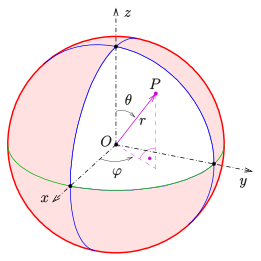
\includegraphics[width=0.5\textwidth]{gps/pictures/kugelkoordinaten.png}
    \caption{Kugelkoordinaten}
%Bild:https://de.wikipedia.org/wiki/Kugelkoordinaten
\end{figure}

\noindent{}Nehmen wir als konkretes Beispiel die Erde. Dann haben wir $r$ als Radius vom Erdmittelpunkt zu dem GPS-Satelliten. $\vartheta$ entspricht den Breitengraden, nur dass diese von oben nach unten gehen bzw. von 0 bis $\pi$. $\varphi$ entspricht dann den Längengraden und geht enstsprechend von 0 bis $\pi$. 

Beschreiben wir eine Position wie z.B. die des Satelliten dann entspricht das $P_{Satellit}(t,r,\vartheta,\varphi)$, wobei $t$ die Zeitkoordinate ist.

\subsubsection{Die Schwarzschildmetrik}
Nun können wir uns die Schwarzschildmetrik zusammen mit den Kugelkoordinaten ansehen. Die Metrik wurde schon als Gleichung in \eqref{skript:kruemmung:schwarzschildmetrik} gezeigt, ist hier aber zur Übersicht nochmal als Matrix dargestellt. \\

\begin{equation}
g_{\mu\nu}= 
\begin{pmatrix}
-\biggl(1-\frac{r_g}r\biggr)c^2 & 0 & 0 & 0 \\
0 & \frac1{\displaystyle 1-\frac{r_g}r} & 0 & 0 \\
0 & 0 &  r^2 & 0 \\
0 & 0 & 0 & r^2 (d\vartheta^2 + \sin^2\vartheta) \\
\end{pmatrix}
\label{skript:gps:schwarzschildmetrik}
\end{equation} \\

\noindent{}$r_g$ entspricht dem Schwarzschildradius, welcher schon in Kapitel \ref{skript:schwarzschild:rg} gezeigt wurde. Zur Übersichtlichkeit wird er hier wieder gezeigt:

\begin{equation}
 r_g=\frac{2MG}{c^2}.
\label{skript:gps:schwarzschildradius}
\end{equation}

\noindent{}Dabei ist \( M = m_{Erde} = 5.972 \cdot 10^{24}\text{kg} \), \( G = 6.673 \frac{Nm^2}{\text{kg}^2} = \) Gravitationskonstante und wie gehabt \( c = 2.9970 \cdot 10^8 \frac{\text{m}}{\text{s}} \). Setzten wir das in die Gleichung \eqref{skript:gps:schwarzschildradius} ein ergibt das folgendes:\\
\begin{align*}
r_g=\frac{2MG}{c^2} = \frac{2 \cdot 5.972 \cdot 10^{24}\text{kg} \cdot  6.673 \frac{Nm^2}{\text{kg}^2}}{ (2.9970 \cdot 10^8 \frac{\text{m}}{\text{s}})^2} = 8.868 \cdot 10^{-3}\text{m} = 8.87\text{mm}
\end{align*}

Wie schon in Kapitel \ref{skript:chapter:schwarzschild} erwähnt, ist dies eine kugelsymmetrische Lösung der Schwarzschildmetrik \eqref{skript:gps:schwarzschildmetrik}. Diese kann als Approximation in der Umgebung von massereichen Objekten benutzt werden, wobei die Eigenrotation der Objekte nicht miteinbezogen ist.

\subsubsection{Die Bahn des Satelliten als Geodäte}
Mit den Kugelkoordinaten können wir die Kreisbahn des Satelliten als Geodäte beschreiben. Rechnet man die Christoffelsymbole für die Schwarzschild-Metrik mithilfe von Maxima o. Ä. aus und setzt diese in die Geodätengleichung ein erhält man folgende Gleichungen:
\begin{align*}
\ddot t(s)
&=
-\frac{1}{1-\displaystyle\frac{r_g}{r}}\frac{r_g}{r}\frac{1}{r}\dot t(s)\,\dot r(s)
\\
\ddot r(s)
&=
-\biggl(1-\frac{r_g}{r}\biggr)\frac{r_g}{r}\frac1{2r}c^2\dot t(s)^2
+\frac{1}{1-\displaystyle\frac{r_g}{r}} \frac{r_g}{r}\frac1{2r}\dot r(s)^2
-(r_g-r)\dot \vartheta(s)^2 + (r_g-r)\sin^2 \vartheta \cdot \dot \varphi(s)^2
\\
\ddot \vartheta(s)
&=
-\frac{2}{r} \dot r(s)\, \dot \vartheta(s)
+\cos\vartheta\sin\vartheta \cdot \dot\varphi(s)^2
\\
\ddot \varphi(s)
&=
-\frac{2}{r} \dot r(s)\,\dot \varphi(s)
-2\cot\vartheta \cdot \dot r(s)\,\dot\varphi(s)
\end{align*}

\noindent{}Diese Gleichungen wurden schon im Kapitel \ref{skript:schwarzschild:geodaetengleichung} hergeleitet. 

Nehmen wir einen Satelliten, der um den Äquator kreist, dann gilt also folgendes:
\begin{align*}
\vartheta &= \frac{\pi}{2} = \text{const} & 
t & = \text{unbek.} & \\
\varphi &= 0..2\pi = \text{unbek.} &
r &= r_{Erde} + h_{Satellit} = \text{const}
\end{align*}

\noindent{}Zum Zeitpunkt $t$ ist die Koordinate $\varphi$ bekannt. Wir haben so eine Beziehung zwischen $t$ und $\varphi$. Wir lassen $t$ und \( \varphi \) daher mal als unbekannt stehen. Wir kennen aber die Koordinaten \(  r \), welche sich aus dem Erdradius und der Höhe des Satelliten zusammensetzen und \( \vartheta \), welches der Äquator ist. Des Weiteren gilt:
\begin{align*}
\dot \vartheta &= 0 & 
\dot r &= 0
\end{align*}

\noindent{}Da $\vartheta = r =$ const sind, sind deren Ableitungen bekanntlich 0.

 Berücksichtigen wir all dies in den Geodätengleichungen, fallen alle Terme mit \( \dot r(s) \) und \( \dot \vartheta (s) \) weg. Des Weiteren fallen die Terme mit \( \cos \vartheta \) weg, denn \( \cos \frac{\pi}{2} = 0 \). Die Geodätengleichungen sehen nun wie folgt aus:
\begin{align*}
\ddot t(s) &= 0 & \implies \dot t &= \text{const.}\\
\ddot r(s)
&=
-\biggl(1-\frac{r_g}{r}\biggr)\frac{r_g}{r}\frac1{2r}c^2\dot t(s)^2
- (r_g-r)\sin^2 \vartheta \cdot \dot \varphi(s)^2 \\
\ddot \vartheta(s) &= 0 \\
\ddot \varphi(s) &= 0 & \implies \dot \varphi & = \text{const.}
\end{align*}

\noindent{}Die einzig aussagekräftige Gleichung die übrig bleibt ist \( \ddot r(s) \). In der Gleichung haben wir sogar eine Beziehung \( \dot t \) und \( \dot \varphi \). Wenn wir die Gleichung noch ewas weiter vereinfachen mit \( \dot r(s) = 0 \implies \ddot r(s) = 0 \) und \( \sin \vartheta = \sin \frac{\pi}{2} = 1 \) dann erhalten wir:

\begin{equation}
0 = -\biggl(1-\frac{r_g}{r}\biggr)\frac{r_g}{r}\frac1{2r}c^2\dot t(s)^2 - (r_g-r)\cdot \dot \varphi(s)^2.
\end{equation}

\subsubsection{Die Vierergeschwindigkeit}
Nun haben wir eine Gleichung aber noch zwei Unbekannte. Um diese zu lösen brauchen wir noch eine zweite. Dazu können wir die Vierergeschwindigkeit als Anfangsbedingung nehmen. Die Vierergeschwindigkeit ist der Ortsvektor abgeleitet nach der Eigenzeit. Es gilt:
\begin{align*}
u &= 
\begin{pmatrix}
t(s) \\
r(s) \\
\vartheta (s) \\
\varphi (s)
\end{pmatrix} &
g_{\mu\nu} &= 
\begin{pmatrix}
-\biggl(1-\frac{r_g}r\biggr)c^2 & 0 & 0 & 0 \\
0 & \frac1{\displaystyle 1-\frac{r_g}r} & 0 & 0 \\
0 & 0 &  r^2 & 0 \\
0 & 0 & 0 &  r^2(d\vartheta^2 + \sin^2\vartheta) \\
\end{pmatrix}
\end{align*}
In unserem Fall entspricht \( u \) der Position des Satelliten und \( g_{\mu\nu} \) der Schwarzschild-Metrik. 

Erinnern wir uns daran, dass die Lichtgeschwindigkeit absolut ist. Möchte man nun von einem Vierervektor seine Länge messen gilt folgende Gleichung, welche in Kapitel \ref{skript:speziell:energieimpuls} schon gezeigt wurde:

\begin{equation}
g_{\mu\nu}u^\mu u^\nu=-c^2 \\
\end{equation}

\noindent{}Das ist eine vom Koordinatensytem unabhängige Grösse. Möchte man eine Längenmessung machen erhält man folgende Gleichung: \\

\begin{equation}
ds^2 = g_{\mu\nu}du^\mu du^\nu = -c^2
\end{equation}

\noindent{}Setzen wir alles ein ergibt sich folgende Gleichung:
\begin{align*}
-\biggl(1-\frac{r_g}r\biggr)c^2 \dot t(s)^2 +  \frac1{\displaystyle 1-\frac{r_g}r} \dot r(s)^2 + r^2 \dot \vartheta(s)^2 + r^2 \dot \vartheta + r^2 \sin^2 \vartheta \dot \varphi (s)^2 = -c^2
\end{align*}

\noindent{}Vereinfachen wir die Gleichung noch, denn \( \dot r(s) = 0 \), \( \dot \vartheta(s) = 0 \) und \( \sin \vartheta = \sin \frac{\pi}{2} = 1 \) dann erhalten wir:
\begin{align*}
-\biggl(1-\frac{r_g}r\biggr)c^2 \dot t(s)^2 + r^2  \dot \varphi (s)^2 = -c^2 
\end{align*}

\noindent{}Und auch hier haben wir wieder eine Beziehung zwischen \( \dot t(s) \) und \( \dot \varphi(s) \). 

\subsubsection{Auflösen des Gleichungsystems}
Jetzt haben wir zwei Gleichungen mit zwei Unbekannten.
\begin{align*}
\RN{1}: &&
0 &= -\biggl(1-\frac{r_g}{r}\biggr)\frac{r_g}{r}\frac1{2r}c^2\dot t(s)^2 - (r_g-r)\cdot \dot \varphi(s)^2
\\
\RN{2}: &&
-c^2  &= -\biggl(1-\frac{r_g}r\biggr)c^2 \dot t(s)^2 + r^2  \dot \varphi (s)^2
\end{align*}

\noindent{}Zuerst vereinfachen wir \RN{1} mit $ (r_g - r) = -r (1 - \frac{r_g}{r} )$.
\begin{align*}
0 &= -\biggl(1-\frac{r_g}{r}\biggr)\frac{r_g}{r}\frac1{2r}c^2\dot t(s)^2 + r (1 - \frac{r_g}{r} ) \dot \varphi(s)^2 && | : \biggr( 1 - \frac{r_g}{r} \biggr)
\\
0 &= -\frac{r_g}{2r^2} c^2 \dot t(s)^2 + r \dot \varphi(s)^2 && | \cdot r
\\
0 &= -\frac{r_g}{2r} c^2 \dot t(s)^2 + r^2 \dot \varphi(s)^2
\end{align*}

\noindent{}Jetzt formen wir \RN{2} nach $ r^2 \cdot \varphi(s)^2$ um.
\begin{align*}
-c^2  &= -\biggl(1-\frac{r_g}r\biggr)c^2 \dot t(s)^2 + r^2  \dot \varphi (s)^2 && | + \biggr( 1 - \frac{r_g}{r} \biggr) c^2 \dot t(s)^2
\\
\biggr( 1 - \frac{r_g}{r} \biggr) c^2 \dot t(s)^2 - c^2 &=  r^2  \dot \varphi (s)^2
\end{align*}

\noindent{}Dann können wir \RN{2} in \RN{1} einsetzen und verinfachen.
\begin{align*}
0 &= -\frac{r_g}{2r} c^2 \dot t(s)^2 + \biggr( 1 - \frac{r_g}{r} \biggr) c^2 \dot t(s)^2 - c^2  && | : c^2
\\
0 &= -\frac{r_g}{2r}\dot t(s)^2 + \biggr( 1 - \frac{r_g}{r} \biggr) \dot t(s)^2 - 1 && | + 1
\\
1 &= -\frac{r_g}{2r}\dot t(s)^2 + \biggr( 1 - \frac{r_g}{r} \biggr) \dot t(s)^2 && \dot t(s)^2 \text{ausklammern}
\\
1 &= \dot t(s)^2 \biggr( -\frac{r_g}{2r} + \biggr( 1 - \frac{r_g}{r} \biggr) \biggr) && \text{Gleichnamig machen}
\\
1 &= \dot t(s)^2 \biggr( \frac{-r_g + 1 - r_g}{2r}\biggr)
\\
1 &= \dot t(s)^2 \biggr( \frac{2r-2r_g}{2r}\biggr)
\\
1 &= \dot t(s)^2 \biggr( \frac{2(r-r_g)}{2r}\biggr) && | r-r_g = r(1-\frac{rg}{r})
\\
1 &= \dot t(s)^2 \biggr( \frac{2r(1-\frac{rg}{r})}{2r}\biggr) && \text{Kürzen}
\\
1 &= \dot t(s)^2 \biggr( 1-\frac{r_g}{r} \biggr) && | : \biggr( 1-\frac{r_g}{r} \biggr)
\\
\frac{1}{1-\frac{r_g}{r}} &= \dot t(s)^2 && | \sqrt{()}
\end{align*}

\noindent{}Und endlich erhalten wir unsere Gleichung für die Zeitdilatation aufgrund der Gravitation:

\begin{equation}
\label{gps:equation:gravidilatation}
\dot t(s) = \tau = \frac{1}{\sqrt{1-\frac{r_g}{r}}}.
\end{equation}

\noindent{}Intressanterweise sieht das sehr ähnlich dem Relativitätsfaktor aus der Gleichung von \ref{eq:realativityfac} aus. Nur das hier nicht die Geschwindigkeit eine Rolle spielt sondern der Abstand zu einem massereichen Objekt. Je grösser die Entfernung zum Objekt desto weniger hat das Gravitationsfeld Einfluss auf die Zeit. 

\subsubsection{Ausrechnen der Zeitdilatation durch Gravitation}
So, jetzt haben wir eine schöne einfache Gleichung und dann können wir nun ausrechnen was für eine Zeitdilatation entsteht durch das Gravitationsfeld.

Die Gleichung \ref{gps:equation:gravidilatation} bezieht sich ja immer auf die Distanz zu einem massereichem Objekt. Genaugenommen zu dem Gravitationszentrum des massereichen Objektes. Das heisst, im Prinzip haben wir auf der Erdoberfläche auch schon eine Zeitdilatation gegenüber dem Erdmittelpunkt. Da sich unsere Position ja grundsätzlich auf der Erdoberfläche befindet müssen wir das auch noch berücksichtigen. Um also die gesamte Zeitdilatation, in Berücksichtigung auf die Erdoberfläche zu erhalten, müssen wir die Zeiltdilatation auf der Erdoberfläche von der Zeitdilatation von dem Satelliten abziehen. Das sieht wie folgt aus:
\begin{align*}
\dot t(s)_ {ges} &= \tau = \frac{1}{\sqrt{1-\frac{r_g}{r_{Erde}}}} - \frac{1}{\sqrt{1-\frac{r_g}{r_{Satellit}}}}
\end{align*}

Die Satelliten kreisen in einer Höhe von 20'200km über der Erdoberfläche. Der Radius ist allerdings auf das Gravitationszentrum bezogen, also müssen wir den Radius der Erde zum Mittelpunkt dazu addieren und dann erhalten wir den gesamt Radius von:
\begin{align*}
r_{Satellit}  = h_{Satellit} + r_{Erde} & = 20.2 \cdot 10^3\text{km} + 6.371 \cdot 10^3\text{km} 
\\
 & = 20.2 \cdot 10^6\text{m} + 6.371 \cdot 10^3\text{m} 
\\
 & = 26.571 \cdot 10^6\text{m}.
\end{align*}

\noindent{}Setzten wir nun diese erlangten Grössen ein erhalten wir:
\begin{align*}
\dot t(s)_ {ges} = \tau & = \frac{1}{\sqrt{1-\frac{r_g}{r_{Erde}}}} - \frac{1}{\sqrt{1-\frac{r_g}{r_{Satellit}}}} = \frac{1}{\sqrt{1-\frac{8.868 \cdot 10^{-3}\text{m}}{ 6.371 \cdot 10^3\text{m}}}} - \frac{1}{\sqrt{1-\frac{8.868 \cdot 10^{-3}\text{m}}{ 26.571 \cdot 10^6\text{m}}}} =  529.09 \cdot 10^{-12}\text{s}
\end{align*}

\noindent{}Das bedeutet nun, dass eine Sekunde auf der Erde \( 529.09\text{ps} \) länger dauert als auf dem Satellit. Je näher man einem massereichem Objekt ist, desto langsamer vergeht die Zeit, abhängig von der Masse des massereichen Objektes. Das entspricht einer Abweichung von 15.9cm pro Sekunde. Rechnet man dies auch wieder auf den ganzen Tag hoch erhält man:
\begin{align*}
t_{tot} & = 529.09 \cdot 10^{-12} \cdot 60 \cdot 60 \cdot 24 = 45.713\frac{\mu{}\text{s}}{\text{d}}
\\
l_{tot} &= 0.3 \cdot 10^{-3} \cdot 60 \cdot 60 \cdot 24 = 13.714\frac{\text{km}}{\text{d}}
\end{align*}

\section{Gesamte Zeitdilatation}
\rhead{Gesamte Zeitdilatation}
Die beiden Effekte haben eine unterschiedliche Wirkung. Als erstes haben wir uns mit der Zeitdilatation durch Geschwindigkeit beschäftigt. Dabei ging es ja darum, dass der Satellit einen Zeitunterschied gegenüber jemandem der sich langsamer oder gar nicht fortbewegt hat. Wegen der höheren Geschwindigkeit des Satelliten gegenüber einem ruhendem Objekt, vergeht dessen Zeit langsamer. Gegenüber die Zeitdilatation durch die Gravitation, welche die Zeit langsamer vergehen lässt je näher man sich einem massereichem Objekt aufhält. Wir auf der Erdoberfläche befinden uns näher am Gravitationszentrum als der Satellit. Das bedeutet gegenüber dem Satelliten verläuft unsere Zeit langsamer. Zusammengefasst heisst das, beim Satelliten läuft die Zeit schneller, da er weiter vom Gravitationszentrum ist, aber wegen seiner Geschwindigkeit wird seine Zeit gebremst.

\begin{equation}
\tau_{tot} = \tau_{Gravitation} - \tau_{Geschwindigkeit}\\
\end{equation}

\noindent{}Wenn man die Zahlen einsetzt erhält man:
\begin{align*}
529.09 \cdot 10^{-12}  -  83.49 \cdot 10^{-12}\text{s} &=  445.6 \cdot 10^{-12}\text{s}
\\
45.713\mu{}\text{s} - 7.213\mu{}\text{s} &= 38.5\frac{\mu{}\text{s}}{\text{d}}
\end{align*}

\noindent{}Das entspricht einer Abweichung von 11.5km pro Tag bzw. 13.37cm pro Sekunde. 

Um diese Zeitdifferenz zu vermeiden, müssen die Satelliten ständig ihre Zeit anpassen. Hätte Einstein nicht die allgemeine Relativitätstheorie entdeckt, hätte man vielleicht nicht verstanden, warum das GPS immer eine falsche Position anzeigt. 

\section{Zahlenspielereien}
\rhead{Zahlenspielereien}
Zurück zu der Frage, wo man im Alltag auf die Effekte der Allgemeinen Relativitätstheorie stösst, das GPS ist ein Beispiel. Das Beispiel zeigt aber auch, dass wenn man nicht eine besonders hohe Geschwindigkeit hat oder sich in der Nähe eines besonders massereichen Objektes befindet, die Effekte extrem klein sind. Sie sind so minimal, dass man sie eigentlich ausser Acht lassen kann. Beim GPS geht das halt nicht, da es tatsächlich nicht klarkommen würde, aber auch für einen Astronauten in der ISS spielt der Effekt keine Rolle. Selbst wenn dieser sich ein paar Jahre auf der Station befindet, und dann zur Erde zurück kehrt ist der Zeitunterschied immernoch sehr sehr klein. Rechnen wir einfach mal ein paar Beispiele durch.

\subsection{Zeitdilatation eines Astronauten der ISS}
Die ISS kreis auf einer durchschnittlichen Orbitalhöhe von \( h_{ISS} = 400\text{km} \). Die ISS ist viel näher als ein GPS Satellit, das heisst der Effekt duch die Gravitation dürfte kleiner sein als dem des Satelliten. Ihre Geschwindigkeit beträgt etwa \( v = 28'000\frac{\text{km}}{\text{h}} = 7777.77\frac{\text{m}}{\text{s}} \). Die Geschwindigkeit hingegen ist viel höher als die des Satelliten, also dürfte hier der Effekt gösser sein. Nutzen wir diese Daten können wir die beiden Zeitdilatationen ausrechen.
\begin{align*}
\tau_{Geschwi} &=  \frac{1}{\sqrt{1 - \frac{v^2}{c^2}}} = \frac{1}{\sqrt{1 - \frac{( 7777.77\frac{\text{m}}{\text{s}})^2}{c^2}}} = 1 + 336.5 \cdot 10^{-12}\text{s}
\\
\tau_{Gravi} &= \frac{1}{\sqrt{1-\frac{r_g}{r_{Erde}}}} - \frac{1}{\sqrt{1-\frac{r_g}{r_{ISS}}}} 
= \frac{1}{\sqrt{1-\frac{r_g}{6371 \cdot 10^3\text{m}}}} - \frac{1}{\sqrt{1-\frac{r_g}{6371 \cdot 10^3\text{m} + 400 \cdot 10^3\text{m}}}} = 41.115 \cdot 10^{-12}\text{s}
\end{align*}

\noindent{}Wieder interessiert uns bei der Dilatation aufgrund der Geschwindigkeit nur die Differenz zu 1. Daraus resultiert eine Gesamtzeitdilatation von:
\begin{align*}
\tau_{ges} = \tau_{Gravi} - \tau_{Geschwi} = -295.3 \cdot 10^{-12}\text{s}
\end{align*}

\noindent{}Hoppla! Was ist denn das für ein Ergebnis. Naja, wenn man sich die Zahlen der beiden Dilatationen anschaut, dann wird einem klar, dass die Gravitation einen kleineren Einfluss hat als die, der Geschwindigkeit. Also kann man hier sagen, dass dem Astronaut Zeit geschenkt wird. Seine Zeit läuft langsamer als die Zeit auf der Erdoberfläche. Rechnet man dies auf einen typisch halbjährigen Aufenthalt in der ISS aus erhält man:
\begin{align*}
-295.3 \cdot 10^{-12} \cdot 60 \cdot 60 \cdot 24 \cdot 180 = -0.00459
\end{align*}

\noindent{}Das ist immer noch weit von einem spürbarem Effekt entfernt. Also selbst für einen Astronauten spielt die Zeitdilatation jetzt durch Geschwindigkeit keine Rolle auch wenn dieser noch viel länger dort bleiben würde.

\subsection{GPS mit Sonne als Gravitationsfeld}
Wir haben bis jetzt immer mit dem Gravitationsfeld der Erde gerechnet. Schauen wir mal was das für das GPS bedeuten würde, wenn unser Planet gleich der Sonne wäre. Zur Sonne haben wir folgende Daten:
\begin{align*}
 m_{Sonne} &= 1.989 \cdot 10^30\text{kg} &  r_{Sonne} &= 6.96 \cdot 10^8\text{m} & r_g &= \frac{2GM}{c^2} = 2.954 \cdot 10^3\text{m}. 
\end{align*}

\noindent{}Gehen wir davon aus dass der Satellit diesselbe Geschwindigkeit hat und die gleiche Höhe. Setzen wir wiederum die Zahlen ein ergibt dies:
\begin{align*}
\tau_{Geschw} &= \frac{1}{\sqrt{1 - \frac{v^2}{c^2}}} = \frac{1}{\sqrt{1 - \frac{3874 \frac{\text{m}}{\text{s}}^2}{(2.9979 \cdot 10^8 \frac{\text{m}}{\text{s}} )^2}}} = 1 + 83.4939 \cdot 10^{-12}\text{s}
\\
\tau_{Gravi} &= \frac{1}{\sqrt{1-\frac{r_g}{r_{Sonne}}}} - \frac{1}{\sqrt{1-\frac{r_g}{r_{Satellit}}}} =  
\frac{1}{\sqrt{1-\frac{2.954 \cdot 10^3\text{m}}{6.96 \cdot 10^8\text{m}}}} - \frac{1}{\sqrt{1-\frac{2.954 \cdot 10^3\text{m}}{ 6.96 \cdot 10^8\text{m} + 20.2 \cdot 10^6\text{m}}}} =  59.85 \cdot 10^{-9}\text{s}
\end{align*}

\noindent{}Die Zeitdilatation aufgrund der Geschwindigkeit bleibt dieselbe. Das ist auch nicht verwunderlich, denn die Zahlen haben sich nicht geändert. Bei der Zeitdilatation wegen der Gravitation hingegen schon. Das ergibt eine gesamt Zeitdilatation von \( \tau_{ges} = 59.85 \cdot 10^{-9}\text{s} = 59.85\text{ns} \), da der Faktor der Geschwindigkeit fast nichts ausmacht. Das sind dann schon 18m pro Sekunde Abweichung nur wegen der Gravitation. Verglichen gegenüber der Erde, bei der die Abweichung nur 2.5cm pro Sekunde beträgt ist das doch eine beachtliche Zahl.

Aber auch hier, die Zeitliche Abweichung ist sehr gering und würde nicht allzuviel ausmachen, auch auf längere Sicht gesehen. Die Effekte sind zwar sehr klein bei nicht sehr massereichen Objekten oder kleinen Geschwindigkeiten spielen die fast keine Rolle. Sind jedoch Systeme von der Zeit abhängig, dann stellt sich die Frage wie genau, bzw.wie ungenau es sein darf. Denn wenn wie beim GPS die Zeit eine sehr grosse Rolle spielt, dann kann es sein, dass man die Allgemeine Relativitätstheorie miteinbeziehen muss.

\subsection{Parker Solar Probe}
Wo wir schon bei der Sonne sind, können wir uns auch die Zeitdilatation der sogennante Parker Solar Probe anschauen. Die Parker Solar Probe ist ein Satellit, der die Sonne ganz nahe Umkreisen soll. Der Satellit wird voraussichtlich am 31. Juli 2018 seinen Start haben. Bei der Umkreisung sollen verschiedenste Daten gesammelt werden. Der Satellit benutzt das sogenannte Swing-by-Manöver. Dabei lässt er sich in das Graviationsfeld der Sonne ``fallen'' um dann der Sonne möglichst nahe zu kommen. Dabei umkreist er dann die Sonne in einer grossen Ellipse. Dieses Manöver wird ein paar mal  ausgeführt. Die maximale Geschwindigkeit, die dabei erreicht wird, wird die höchste bis dahin erreichte Geschwindigkeit, welche je von einem Menschen geschaffenem Objekt erreicht wurde. Wir schauen uns die Extremfälle an und schauen, welche Zeitdilatationen dort auftauchen. Zum einen ist dies, wenn der Satellit der Sonne am nächsten ist und zum anderen, wenn der Satellit der Sonne am weitesten entfernt ist. Wir betrachten nur die Situation bei dem Swing-by-Manöver, sonst wäre die weiteste Distanz, dieselbe zur Erde und das wäre ziemlich uninteressant. 

\subsubsection{Zeitdilatation aufgrund der Geschwindigkeit}
Da der Satellit in einer Ellipse um die Sonne kreisen wird, wird er zu jedem Zeitpunkt eine andere Geschwindigkeit haben. Das wird klarer bei einer bildlichen Darstellung.
\begin{figure}[h]
    \centering
    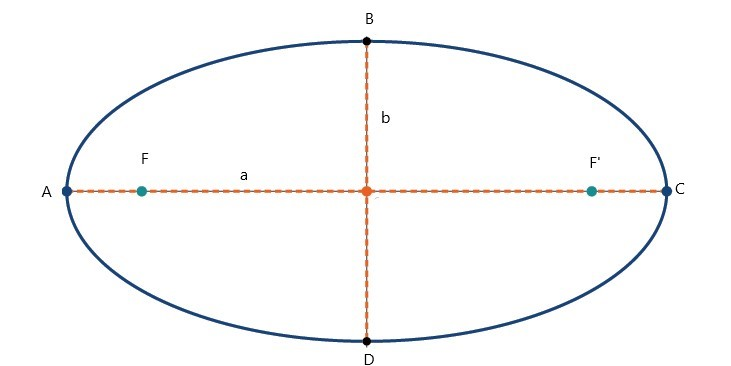
\includegraphics[width=0.75\textwidth]{gps/pictures/Ellipse.jpg}
    \caption{Ellipse}
    \label{pic:ellipse}
%Bild:http://philschatz.com/precalculus-book/resources/CNX_Precalc_Figure_10_01_004.jpg
\end{figure}

\noindent{}Der Punkt F stellt die Sonne und somit das Gravitationszentrum dar. Der Punkt F' ist das theoretische andere Gravitationszentrum. Die Punkte A und C sind die Extrempunkte denen wir uns widmen. Für das weitere Verständnis noch ein paar Begriffserklärungen. Die Strecke $\overline{AF}$ wird Periapsis genannt und die Strecke $\overline{FC}$ Apsis. a ist die Strecke von A bis zum Mittelpunkt und wird grosse Halbachse genannt und b ist die Strecke B bis zum Mittelpunkt und ist die kleine Halbachse.

Da der Satellit bei A der Sonne am nächsten ist, ist die Geschwindigkeit am grössten. Bei C ist es hingegen die kleinste. Um die Geschwindigkeiten dort herauszufinden brauchen wir die Vis-Viva-Gleichung, welche gleich erläutert wird.

\subsubsection{Einfache Herleitung der Vis-Viva-Gleichung}
Die Vis-Viva-Gleichung lässt uns zu jedem Zeitpunkt in der elliptischen Umkreisung des Satelliten die Geschwindigkeit berechnen. Um die Gleichung zu verstehen gibt es eine vereinfachte Herleitung. Wir müssen uns bewusst sein, dass der Satellit die Sonne in einer elliptischen Bahn umkreist. Aufgrund dessen verändert sich seine Geschwindigkeit je nach Position. 

\subsubsection{Energiesatz}
Betrachten wir den Energiesatz, bleibt die gesamt Energie des Satelliten immer die gleiche. Diese setzt sich aus der kinetischen und der potentiellen Energie zusammen.
\begin{equation}
E = E_{pot} + E_{kin}
\end{equation}

\noindent{}Dabei berechnet sich die potentielle Energie nach dem klassischem Newton'schen Gravitationsgesetz.
\begin{equation}
E_{pot} = F(x) = G\frac{Mm}{x^2}
\end{equation}

\noindent{}Dabei gilt x dem Abstand zum Gravitationszentrum und G entspricht der Gravitationskonstante und M der Masse des Objektes, welches umkreist wird. Da sich dieser auf der Bahn immer wieder ändert, ändert sich auch dessen Potential. Integrieren wir entlang einem Radius $r_0$ nach $r$ erhalten wir die Differenz des Potentials. 
\begin{align*}
\int_{r_0}^{r} F(x) dx= \int_{r_0}^{r} G\frac{Mm}{x^2} dx = GMm \int_{r_0}^{r} \frac{1}{x} dx = GMm \biggr( \frac{1}{r_0} - \frac{1}{r}\biggr)
\end{align*}

\noindent{}Somit gilt für die gesamt Energie:
\begin{align*}
E = E_{pot} + E_{kin} = GMm \biggr( \frac{1}{r_0} - \frac{1}{r}\biggr) + \frac{1}{2}mv^2
\end{align*}

\noindent{}Nehmen wir zwei Punkte, wie zum Beispiel A und C aus Abbildung \ref{pic:ellipse}, müssen deren Energie gleich sein.
\begin{align*}
GMm \biggr( \frac{1}{r_A} - \frac{1}{r}\biggr) + \frac{1}{2}mv_A^2 = GMm \biggr( \frac{1}{r_C} - \frac{1}{r}\biggr) + \frac{1}{2}mv_C^2
\end{align*}

\noindent{}Noch ein bisschen vereinfacht und nach $v_A$ umgestellt:
\begin{align*}
GM \biggr( \frac{1}{r_A} - \frac{1}{r}\biggr) + v_A^2 &=  GM \biggr( \frac{1}{r_A} - \frac{1}{r}\biggr) + v_C^2
\end{align*}

\begin{equation}
v_A^2 = v_C^2 + 2GM \biggr( \frac{1}{r_A} - \frac{1}{r_C}\biggr)
\label{eq:keplerenergie}
\end{equation}

\subsubsection{Keplers zweites Gesetz}
Das zweite Keplersche Gesetz besagt, dass wenn sich ein
 Objekt in einer elliptischen Umlaufbahn sich eine bestimte Zeit bewegt und ein zweites Objekt sich an einer anderen Position der Umlaufbahn sich die gleiche Zeit lang bewegt, die Fläche der Dreiecke, die sich zum Graviationszentrum bilden, gleich gross sind.
\begin{figure}[h]
    \centering
    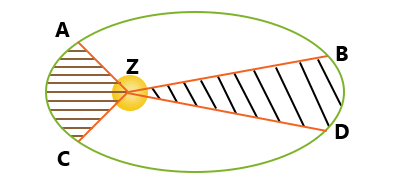
\includegraphics[width=0.5\textwidth]{gps/pictures/keplersec.png}
    \caption{Gleiche Fläche}
%Bild:http://images.tutorvista.com/cms/images/147/keplers-second-law.png
\end{figure}

\noindent{}Die Dreiecke ACZ und BZD sind gleich gross, wenn die vergangene Zeit auf dem Umlaufbahn diesselbe ist. Betrachten wir das linke Dreieck mal genauer.
\begin{figure}[H]
    \centering
    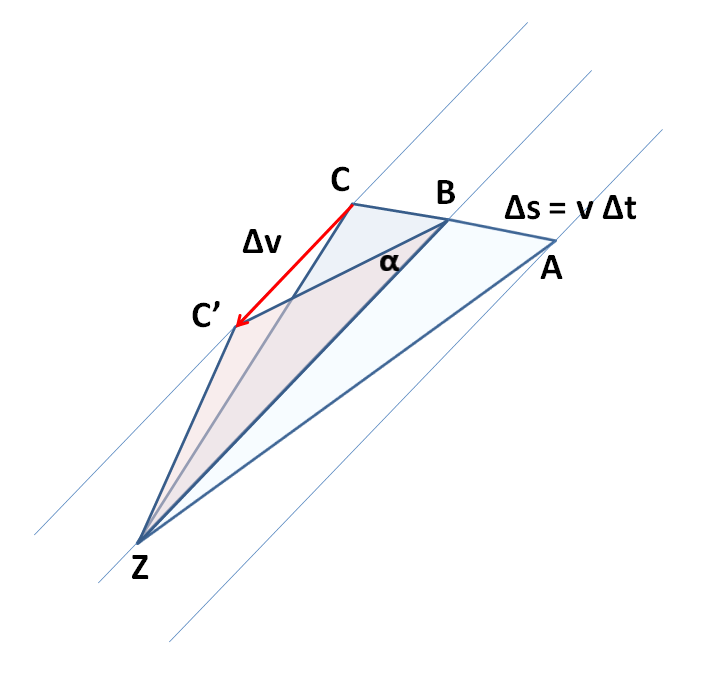
\includegraphics[width=0.5\textwidth]{gps/pictures/KeplerArea.png}
    \caption{Grösse der Fläche}
    \label{pic:flaeche}
%Bild:https://de.wikipedia.org/wiki/Keplersche_Gesetze#/media/File:Kepler2.png
\end{figure}

\noindent{}Eigentlich würde sich das Objekt von A nach B nach C bewegen, wird aber durch das Gravitationszentrum bei B nach C' abgelenkt. Die Strecke $\overline{CC'}$ entspricht dem $\Delta v$. Die Strecke $\overline{AB}$ entspricht $v \Delta t$. Und da die Strecke $\overline{ZB}$ parallel zu $\Delta v$ ist entspricht die Höhe des Dreiecks C'ZB der Strecke $v \Delta t$. Der Winkel C'BZ sei $sin(\alpha)$. Möchten wir also die Fläche C'ZB berechnen, dann entspricht dies:
\begin{align*}
A = \frac{1}{2} hr = \frac{1}{2} v \cdot \Delta t \cdot \sin(\alpha) \cdot r
\end{align*}

\noindent{}Je kleiner $\Delta t$ wird desto kleiner wird $\Delta v$ und der Winkel $\alpha$ wird grösser. Denken wir wieder an die Extrempunkte A und C aus Abbildung \ref{pic:ellipse}. An diesen Punkten und wenn $\Delta t$ sehr klein ist (sprich $\sin (\alpha) = \sin(90\degree) = 1$) gilt, da beide Flächen gleich sein müssen:
\begin{align*}
\frac{1}{2} v_A \cdot \Delta t \cdot \sin(\alpha) \cdot r_A &= \frac{1}{2} v_C \cdot \Delta t \cdot \sin(\alpha) \cdot r_C
\end{align*}

\noindent{}Was wir noch vereinfachen können.
\begin{equation}
v_A \cdot r_A = v_C \cdot r_C \implies v_C = \frac{v_A \cdot r_A}{r_C}
\label{eq:kepler}
\end{equation}

\subsubsection{Vis-Viva-Gleichung}
Da der Punkt A zum Gravitationszentrum dem Radius $r_A$ entspricht und C zum Gravitationszentrum dem Radius $r_C$ sind die beiden in der Summe gleich zwei mal die grosse Halbachse.
\begin{equation}
2a = r_A + r_C \implies r_C = 2a - r_A
\label{eq:ellips}
\end{equation}

Jetzt können wir alles zusammensetzen. Nutzen wir die Gleichung \eqref{eq:keplerenergie} und setzen \eqref{eq:kepler} und \eqref{eq:ellips} ein und vereinfachen alles, erhalten wir:
\begin{equation}
v(r) = \sqrt{GM \biggr(\frac{2}{r} - \frac{1}{a}\biggr)}
\label{visvivagleichung}
\end{equation}

\subsubsection{Berechnung der Zeitdilatation aufgrund der Geschwindigkeit}
Jetzt können wir die Zeitdilatation aufgrund der Geschwindigkeit berechnen. Wir haben:
\begin{align*}
M &= 1.989 \cdot 10^30\text{kg} & r_A & = 6\cdot 10^3\text{km} & r_C &= 109.3\cdot 10^3\text{km}
\end{align*}
\begin{align*}
a &= \frac{r_A + r_C}{2} = \frac{6\cdot 10^6\text{km} + 109.3\cdot 10^6\text{km}}{2} = 57.65\cdot 10^6 \text{km}
\end{align*}

\noindent{}Setzen wir die Zahlen ein:
\begin{align*}
v(r_A) & = \sqrt{GM \biggr(\frac{2}{r_A} - \frac{1}{a}\biggr)} 
\\
& = \sqrt{6.674 \cdot 10^{-11}\frac{\text{Nm}^2}{\text{kg}^2} \cdot 1.9889 \cdot 10^{30}\text{kg} \biggr(\frac{2}{6\cdot 10^6\text{km}} - \frac{1}{57.65\cdot 10^6 \text{km}}\biggr)} = 204.802 \frac{\text{km}}{\text{s}}
\\
v(r_C) & = \sqrt{GM \biggr(\frac{2}{r_C} - \frac{1}{a}\biggr)} \\
& = \sqrt{6.674 \cdot 10^{-11}\frac{\text{Nm}^2}{\text{kg}^2} \cdot 1.9889 \cdot 10^{30}\text{kg} \biggr(\frac{2}{109.3\cdot 10^6\text{km}} - \frac{1}{57.65\cdot 10^6 \text{km}}\biggr)} = 11.242 \frac{\text{km}}{\text{s}}
\\
\end{align*}

\noindent{}Setzen wir diese Zahlen in die Gleichung \eqref{eq:realativityfac} erhalten wir:
\begin{align*}
\tau_{r_A} & = \frac{1}{\sqrt{1 - \frac{v_{p}^2}{c^2}}} = \frac{1}{\sqrt{1 - \frac{(204.802 \frac{\text{km}}{\text{s}})^2}{c^2}}} = 1 + 233.19 \cdot 10^{-9}
\\
\tau_{r_C} & = \frac{1}{\sqrt{1 - \frac{v_{a}^2}{c^2}}} = \frac{1}{\sqrt{1 - \frac{(11.242 \frac{\text{km}}{\text{s}})^2}{c^2}}} =  1 + 703 \cdot 10^{-12}
\end{align*}

\subsubsection{Zeitdilatation aufgrund des Gravitationsfeldes}
Wir haben:
\begin{align*}
 r_{Sonne} &= 6.96 \cdot 10^8\text{m} & r_g &= \frac{2GM}{c^2} = 2.954 \cdot 10^3\text{m}
\\
r_A & = 6\cdot 10^{12}\text{m} & r_C &= 109.3\cdot 10^{12}\text{m}
\end{align*}

\noindent{}Setzen wir die Zahlen ein:
\begin{align*}
\tau_{r_A} &= \frac{1}{\sqrt{1-\frac{r_g}{r_{Sonne}}}} - \frac{1}{\sqrt{1-\frac{r_g}{r_{r_A}}}} =  
\frac{1}{\sqrt{1-\frac{2.954 \cdot 10^3\text{m}}{6.96 \cdot 10^8\text{m}}}} - \frac{1}{\sqrt{1-\frac{2.954 \cdot 10^3\text{m}}{ 6\cdot 10^{12}\text{m} }}} =  2.1219 \cdot 10^{-6}\text{s}
\\
\tau_{r_C} &= \frac{1}{\sqrt{1-\frac{r_g}{r_{Sonne}}}} - \frac{1}{\sqrt{1-\frac{r_g}{r_{r_C}}}} =  
\frac{1}{\sqrt{1-\frac{2.954 \cdot 10^3\text{m}}{6.96 \cdot 10^8\text{m}}}} - \frac{1}{\sqrt{1-\frac{2.954 \cdot 10^3\text{m}}{ 109.3\cdot 10^{12}\text{m} }}} =  2.1221 \cdot 10^{-6}\text{s}
\end{align*}

\noindent{}Interessanterweise unterscheiden sich die Zahlen nicht gross.

\subsubsection{Gesamte Zeitdilatation an den Extrempunkten}
Jetzt können wir die gesamte Zeitdilatation ausrechnen:
\begin{align*}
\tau_{r_A} & = \tau_{Gravi_{r_A}} - \tau_{Geschw_{r_A}} = 2.1219 \cdot 10^{-6}\text{s} - 233.19 \cdot 10^{-9} = 2.1219 \cdot 10^{-6}\text{s}
\\
\tau_{r_C} & = \tau_{Gravi_{r_C}} - \tau_{Geschw_{r_C}} = 2.1221 \cdot 10^{-6}\text{s} - 703 \cdot 10^{-12} = 2.1221 \cdot 10^{-6}\text{s}
\end{align*}

\noindent{}Der Effekt aufgrund der Geschwindigkeit ist gegenüber der Gravitation viel kleiner und kann vernachlässigt werden. Aber gesamthaft gesehen sind es doch etwas mehr als 2$\mu$s (!) Abweichung pro Sekunde. Auf den Tag gesehen sind dies:
\begin{align*}
2.12 \cdot 10^{-6}\text{s} \cdot 60 \cdot 60 \cdot 24 = 0.183\text{s}
\end{align*}
\noindent{}Das ist doch extrem viel verglichen mit den anderen Beispielen.

\printbibliography[heading=subbibliography]
\end{refsection}